\documentclass[letterpaper]{article}

\usepackage[utf8]{inputenc}
\usepackage[sort, colon]{natbib}
\usepackage{alifexi}
\usepackage[bottom]{footmisc}
\usepackage[colorlinks=true,citecolor=green,linkcolor=blue]{hyperref}
\usepackage[font=scriptsize,labelfont=bf]{caption}
\usepackage{tabulary}

\usepackage{mathtools}
\usepackage{commath}

\usepackage{dblfloatfix}

\title{Reproducing and updating results from
\textit{Uncovering disease-disease relationships\\through the incomplete interactome}}
\author{Robin Petit$^{1}$ \and Tom Lenaerts$^{1}$\\
\mbox{}\\
$^1$Université Libre de Bruxelles}


\begin{document}
\maketitle

\begin{abstract}
  This paper intends to reproduce the results exposed of the article \textit{Uncovering
	disease-disease relationships through the incomplete interactome} \citep{originalPaper}
	and check the robustness of the procedure by confronting the results with the results of
	updated datasets, which intends to be a systematic analysis, still stands for a more
	recent version of the interactome, and if the results exposed have shifted towards a more
	or less significant level. We find that besides being reproducible, some of the results
	exposed turn out to be more significant, and others turn out to be less significant.
\end{abstract}

\section{Introduction}
An interactome is a graph containing all the molecular interactions within a cell. This notion appeared
in 1999 (for the drosophila) \citep{sanchez1999grasping} and the need to thoroughly study this structure has
been expressed less than 15 years ago \citep{UnderstandingTheCellFunctionalOrganization}.

The interactome is one of the many biological networks, covering gene networks also called genome,
protein networks also called proteome \citep{rolland2014proteome}, disease networks \citep{goh2007human} among
others, and providing the ability to deeply study biology \citep{UnderstandingTheCellFunctionalOrganization} as
well as medicine \citep{barabasi2011network} or more recently pharmacology \citep{hopkins2008network}.

As the need to use the interactome as a tool to analyze diseases genetic behaviour had already been
expressed \citep{vidal2011interactome}, the authors or the original paper \citep{originalPaper} showed
that the human interactome has now reached sufficient completion to systematically study diseases. Yet,
the interactome provides the availability to study many more genetic relations, such as drug-disease
correlation \citep{Yu2016extraction}, or digenic diseases \citep{gazzo2015dida}.

In the original paper, authors applied disease genes association databases (in particular
OMIM, the Online Mandelian Inheritance in Man \citep{amberger2008OMIM}, and GWAS, the Genome-Wide Association
Studies, compiled by PhenGenI \citep{ramos2014PhenGenI}) on the human interactome in order to determine
the properties of their distribution in the graph.

The diseases studied are selected such that they possess at least 20 genes associated to them, which yields
29,775 disease-gene associations on 3,173 distinct genes, with 2,436 contained in the interactome.

Major results were that: firstly diseases tend to \textit{cluster} in denser subgraphs than the
interactome itself (shown by bigger largest connected component than expected in random interactome
subgraphs), secondly that phenotypically close diseases tend to overlap on a significant amount of genes.

Authors of the original paper also remind that the interactome is incomplete and estimated around $20\%$-complete
for the interactions by the estimation that the interactome contains roughly $6.5 \times 10^5$ interactions,
and around $54\%$-complete for the proteins involved by the estimations that the interactome contains roughly
$2.5 \times 10^4$ nodes \citep{ATruerMeasureOfOurIgnorance,estimatingTheSizeOfTheHumanInteractome}

The first part of this paper focuses on the reproduction of exposed results in the original paper,
namely the disease modules propensity to cluster into highly connected components and the significantly
lower separation indicator values for highly gene related disease pairs.

The interactome used in the original paper contains 13,460 genes and 141,296 physical links constructed on several
interactions databases including BioGRID \citep{chatr2017biogrid}, IntAct \citep{kerrien2011intact},
TRANSFAC \citep{matys2003transfac}, MINT \citep{licata2011mint}, HPRD \citep{keshava2008HPRD}, KEGG and
BIGG \citep{lee2008KEGG-BIGG}, CORUM \citep{ruepp2009corum} and PhosphitePlus \citep{hornbeck2011phosphositeplus}.
Authors chose to rely only on physical protein-protein interactions (PPI) and to exclude functional interactions
\citep{caldera2017interactome}. This interactome is available to download as supplementary material.

\section{Results}
	\subsection{Reproducibility}
		\subsubsection{Clustering of disease modules}\label{subsec:clustering of disease modules}
		The original paper discusses the trend of diseases to cluster into dense subgraphs. In order to measure
		this hypothesis, the largest connected component (LCC) of the diseases in the interactome is used.
		When analyzing this, we observe that 241 out of the 299 diseases (more than $80\%$) have a significantly
		bigger LCC than expected by chance.

		The $z$-score of the LCC size of a disease is strongly related to its relative module size, which is
		defined by $r = S/N_d$, with $S$ the size of the LCC of the disease, and $N_d$, the number of genes
		associated with the given disease (Figure~\ref{fig:zscore}).

		\begin{figure}[!h]
			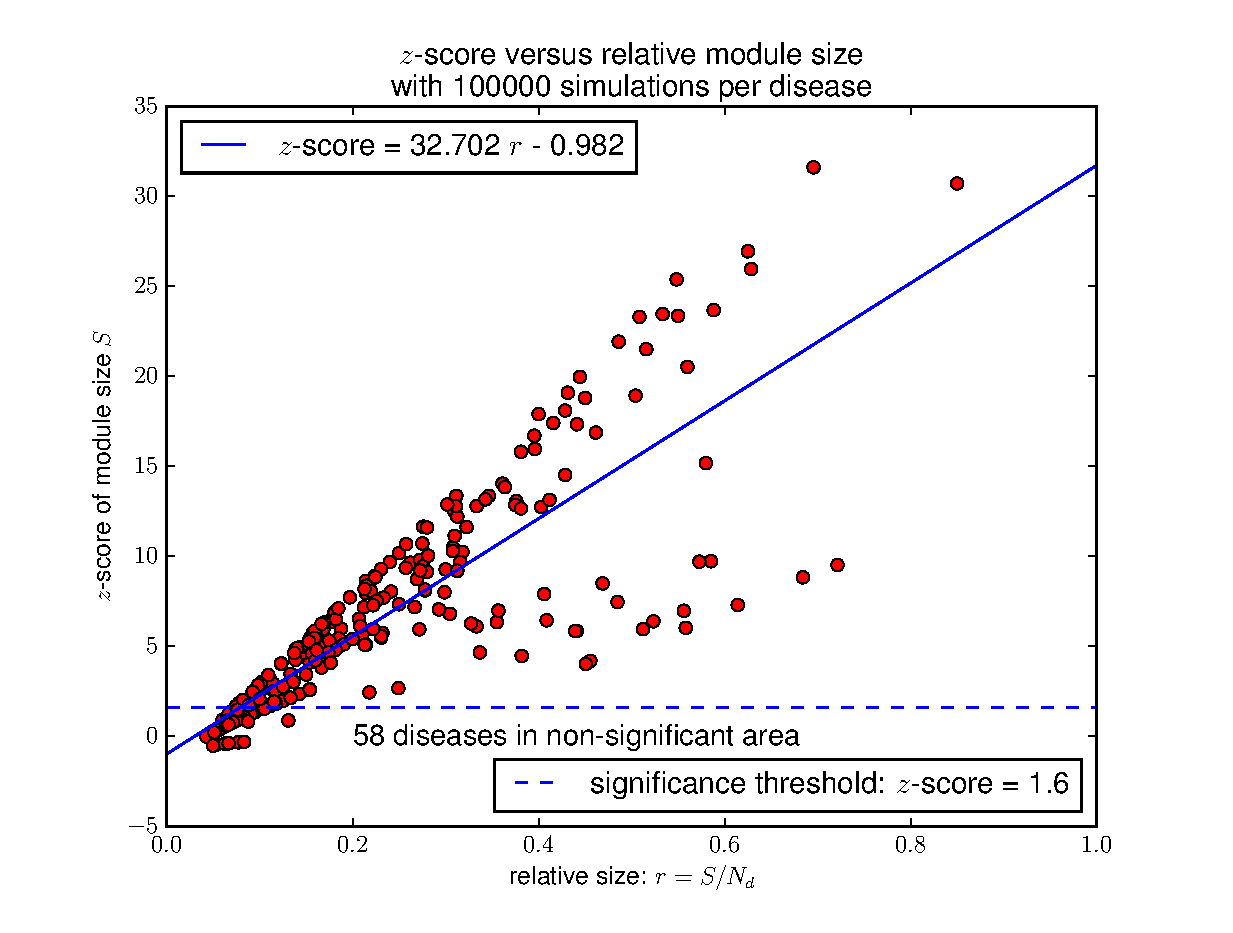
\includegraphics[width=.5\textwidth]{images/S4.b100000.eps}
			\caption{\textbf {$z$-score of largest connected component size vs relative module size.}
			100,000 simulations have been performed per disease in order to determine the size of the largest connected component
			of the disease subgraph expected by chance. Diseases being highly connected (thus highly covered by the interactome)
			present a higher $z$-score and then a higher confidence about the significance of the size difference.
			Assuming that the distribution of largest connected component is normal for random
			samples \citep{fluctuationGiantComponent}, each $z$-score can be associated to a $p$-value, in particular,
			$z$-score $\geq 1.6$ corresponds to $p$-value $\leq 0.05$, representing significance threshold. \label{fig:zscore}}
		\end{figure}

		This allows to observe that several diseases do not present a significantly larger largest connected component
		than expected by chance, but that these diseases have a thin relative size ($< 0.2$, so that less than $20\%$
		of their related genes are connected in the current interactome). Also, diseases with bigger relative size
		have a higher $z$-score, leading to think that a more complete interactome, with higher coverage of the diseases
		would increase the significance of the result.

		\subsubsection{Separation distribution}
		The original paper describes the separation of diseases in the interactome through two different measures:
		the overlapping score ($C$-score and $J$-score defined respectively as $\abs {A \cap B}/\min(\abs A, \abs B)$
		and $\abs {A \cap B}/\abs {A \cup B}$ for $A$ and $B$ two disease genes sets) and the separation score $s_{AB}$
		defined as follows. For two diseases $A$ and $B$, let $\langle d_A \rangle$ and $\langle d_B \rangle$ be the mean
		distance between two proteins in the disease subgraphs of $A$ and $B$ respectively, and let $\langle d_{AB} \rangle$
		be the mean distance between two proteins of each disease subgraph. Then define $s_{AB}$ as:
		\begin{equation}
			s_{AB} = \langle d_{AB} \rangle - \frac {\langle d_A \rangle + \langle d_B \rangle}{2}.
		\end{equation}

		Table~\ref{tab:J-C-scores} details the meaning of $J$/$C$-scores combinations.

		\begin{table}
		\begin{tabular}{m{.1\textwidth}|m{.1\textwidth}|m{.08\textwidth}|m{.08\textwidth}}
			$J = 0$ & $0 < J < 1$ & $J < 1$ & $J = 1$ \\
			$C = 0$ & $0 < C < 1$ & $C = 1$ & $C = 1$ \\
			\hline
			\hline
			No common gene & Partial overlap & $A$ is complete subset of $B$ & $A$ and $B$ are identical
		\end{tabular}
		\caption{Meaning of the different $J$-score/$C$-score combinations.\label{tab:J-C-scores}}
		\end{table}

		When analyzing the separation of the interactome, we find out the same results than those presented in the
		original article. The only difference being that for non-overlapping disease pairs, the amount of pairs
		having a separation value below 0 is $710$ versus $717$ in the original paper, being totally non-significant
		since $7$ pairs represent less than $0.03\%$ of all the non-overlapping pairs set (Figure~\ref{fig:s_AB histogram}).

	\subsection{Robustness}

		\subsubsection{Databases update}
		In order to update the interactome, the tool \textit{inter-tool} \citep{inter-tools} has been used.
		Latest datasets from BioGRID, IntACT, and the Database of Interacting Proteins (DIP) \citep{salwinski2004DIP}
		(on July 25th) and of MINT (on July 27th) have been downloaded and merged via inter-tools.

		This newer version merged with the original interactome yields a new graph having 17,786 nodes and 370,326 edges
		(so a bit more than 1.3 times the initial amount of nodes, and more than 2.6 times the initial amount of edges).
		From the 4326 genes added in this newer version, 361 are associated with one of the 299 diseases, leading to 2,797
		disease-associated genes in the interactome.


		\begin{figure}[!h]
			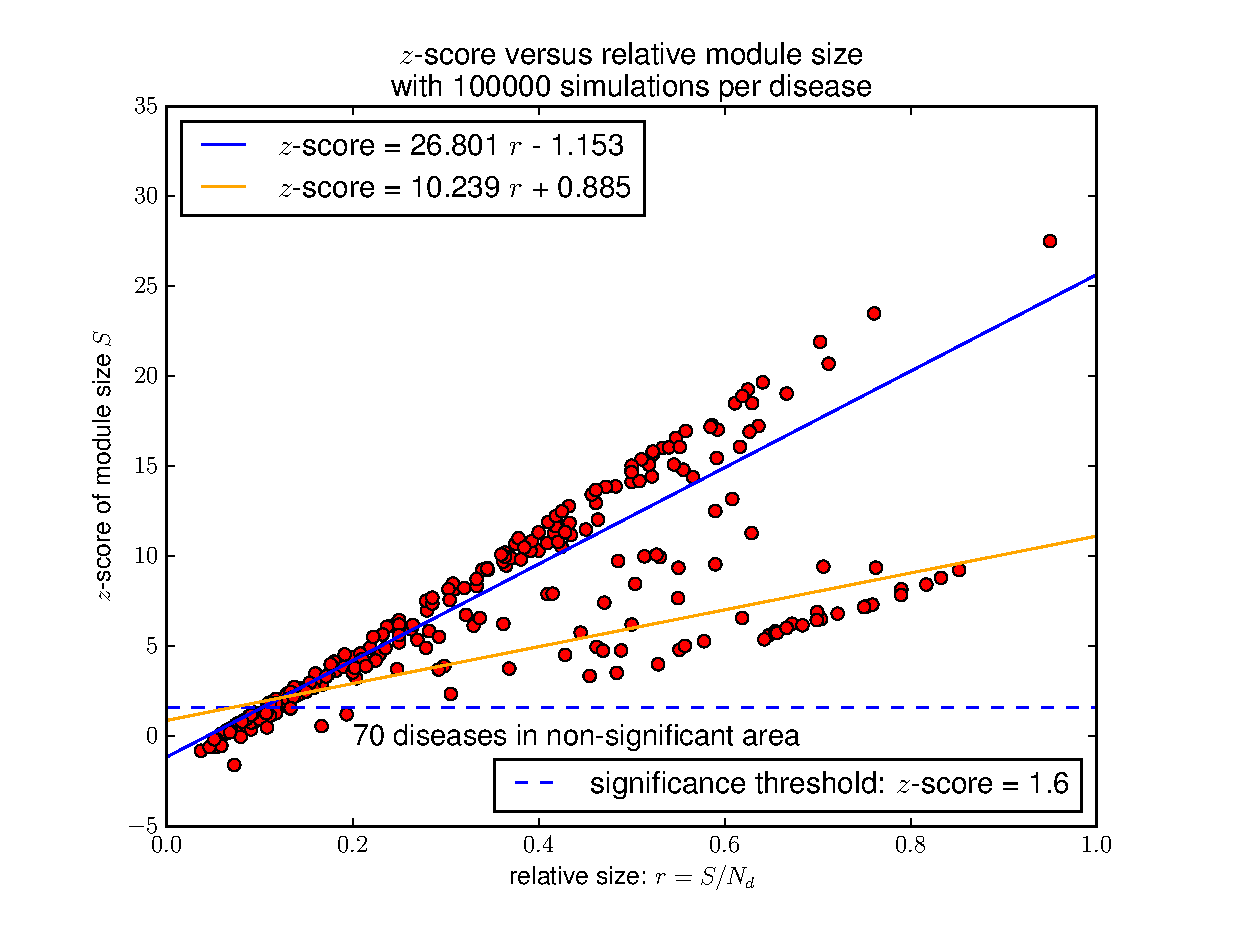
\includegraphics[width=.5\textwidth]{images/new_interactome_S4.b100000.eps}
			\caption{{\bf z-score of the largest connected component size vs relative module size of the newer interactome.}
			Adaptation of Figure~\ref{fig:zscore} on the newer version of the interactome.
			\label{fig:new interactome zscore}}
		\end{figure}

		\begin{figure*}[!t]
			\hspace{-1.8cm}
			\vspace{-1cm}
			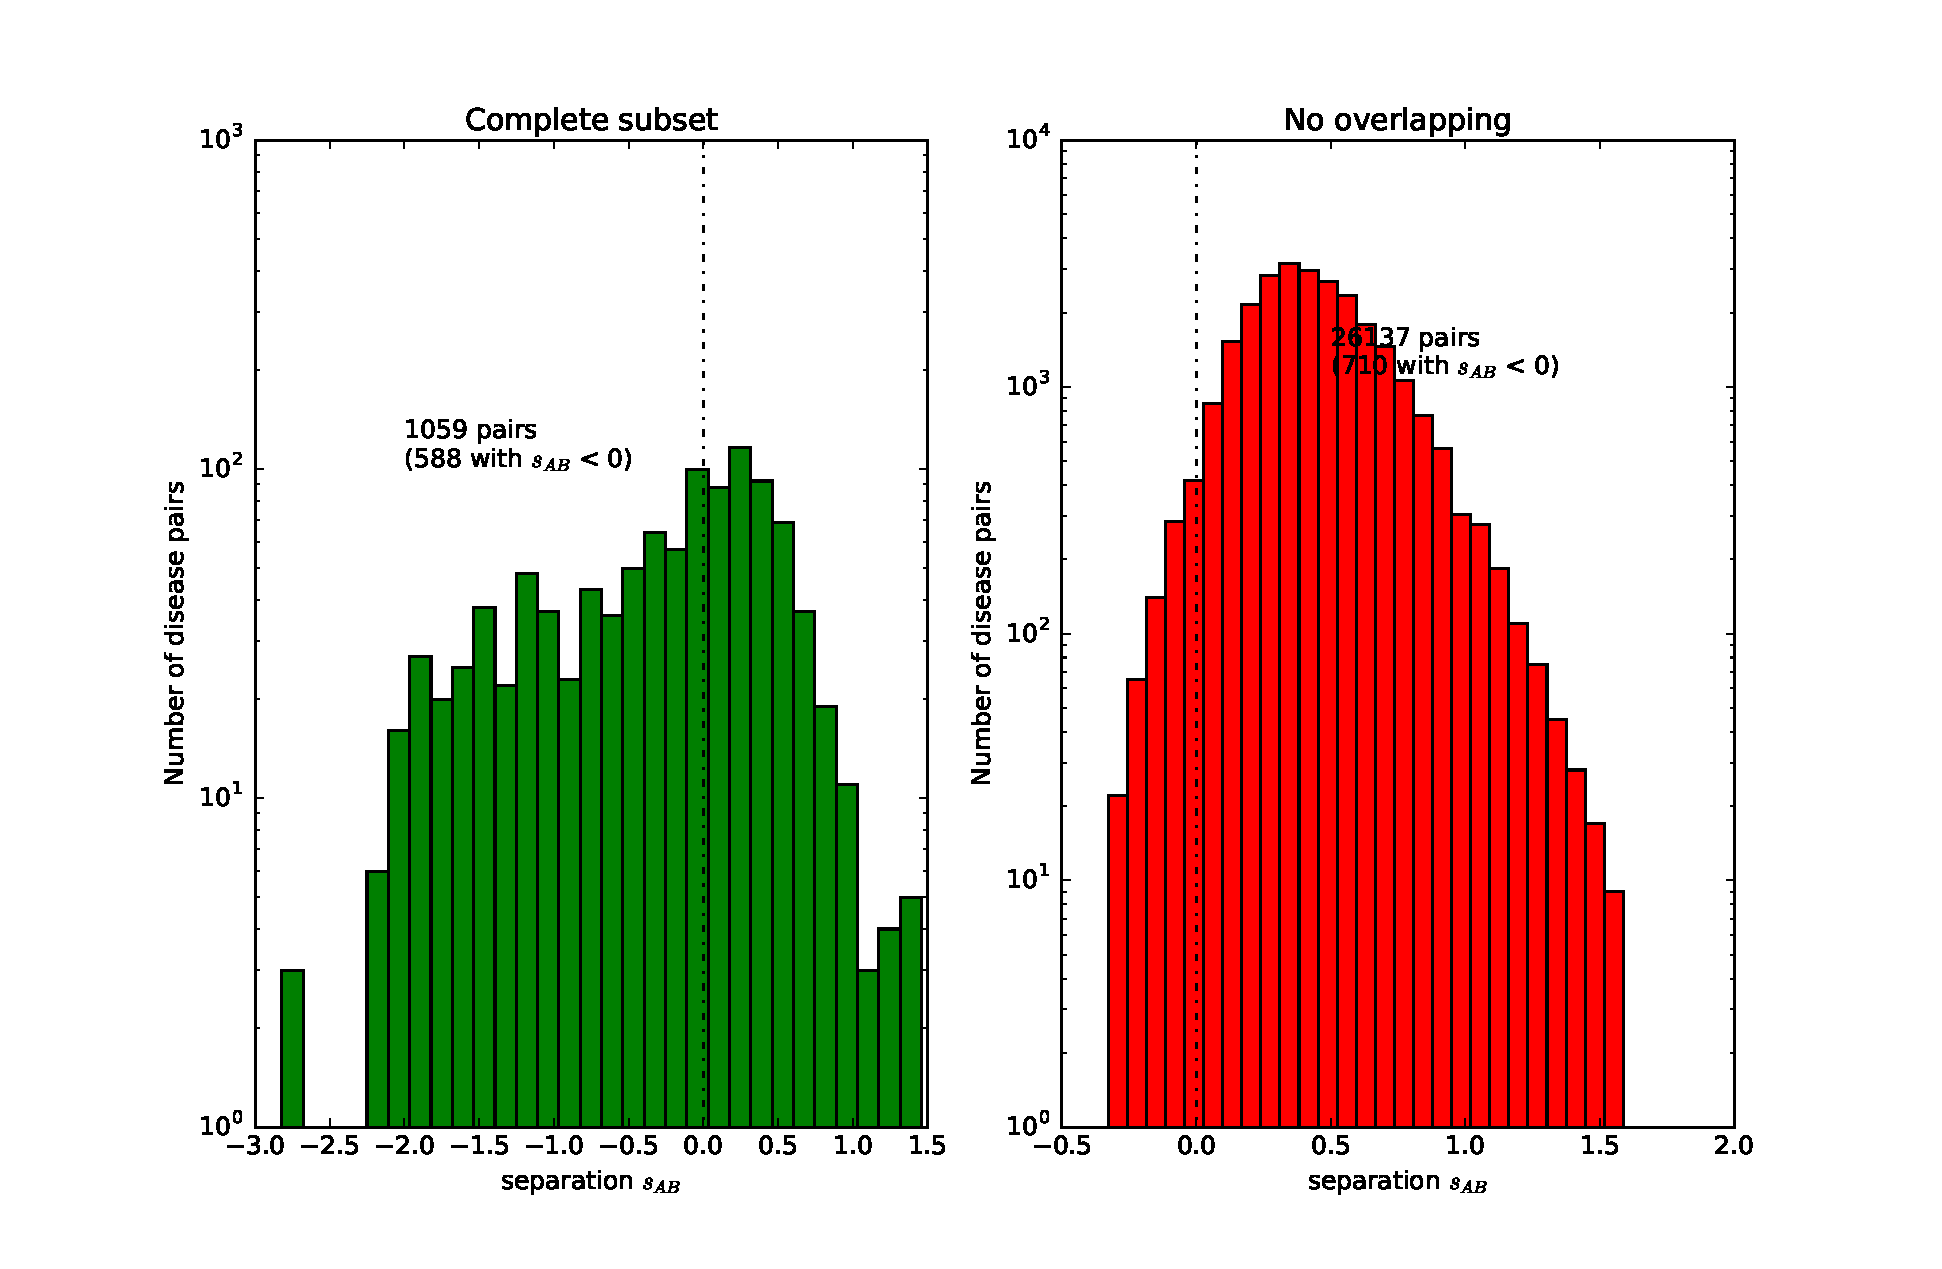
\includegraphics[scale=.35]{images/s_AB_histograms.eps}
			\caption{\label{fig:s_AB histogram}
			{\bf Disease pairs separation.}
			({\bf A}) The $s_{AB}$ distribution of disease pairs with no common gene ($C$-score = $J$-score $= 0$). We
			observe that even though no gene is shared, 710 of the 26,137 pairs (less than $3\%$) have a negative
			separation score (between 0 and 0.5).
			({\bf B}) The $s_{AB}$ distribution of disease pairs with complete overlap ($J$-score $< C$-score $= 1$).
			We observe that despite the inclusion of one disease genes set in the other, 471 of the 1,101 pairs
			(more than $42\%$) have a positive separation score. Yet, separation goes to very low values (below 2).
			({\bf C}) The $s_{AB}$ distribution of disease pairs partially overlapping ($0 < J$-score $ \leq J$-score $< 1$).
			These disease pairs show the same spike of frequency right to $s_{AB} = 0$ as in (A) and the same tail of frequency
			left to $s_{AB} = 0$.
			({\bf D}) The $s_{AB}$ distribution of all the disease pairs.
			}
		\end{figure*}

		This newer version is around $71\%$-complete for the proteins involved and $57\%$-complete for the
		interactions \citep{estimatingTheSizeOfTheHumanInteractome,ATruerMeasureOfOurIgnorance}.

		Disease genes considered in this update are the same 299 diseases studied in the original paper. An update of these
		is yet to be done in further investigations.

	\subsection{Discussion}
	By defining the density of a graph $\Gamma = (V, E)$ as being $d(\Gamma) \coloneqq \abs E/\binom {\abs V}2$,
	we find that the newer interactome is more than 1.5 times denser than the original one ($0.156\%$ versus $0.234\%$
	for the newer one).

	When performing the same localization analysis of the disease modules in the interactome on the newer version,
	we observe that 12 more diseases have a $z$-score below the threshold of $1.6$, which makes results less significant
	(Figure~\ref{fig:new interactome zscore}).

	\begin{figure}[!h]
		\includegraphics[width=.5\textwidth]{images/rel_sizes_comparison.eps}
		\caption{{\bf Comparison of relative size distribution between original and newer interactomes.}
		We observe that the number of diseases having a relative size below $\simeq 0.35$ has lowered, whereas the number
		of diseases having a relative size above $\simeq 0.35$ has increased. This is explained by the bigger density of
		the newer interactome, leading to larger LCC in the disease subgraphs.
		\label{fig:rel sizes comparison}}
	\end{figure}

	\begin{figure*}[!b]
		\hspace{-1.8cm}
		\vspace{-.5cm}
		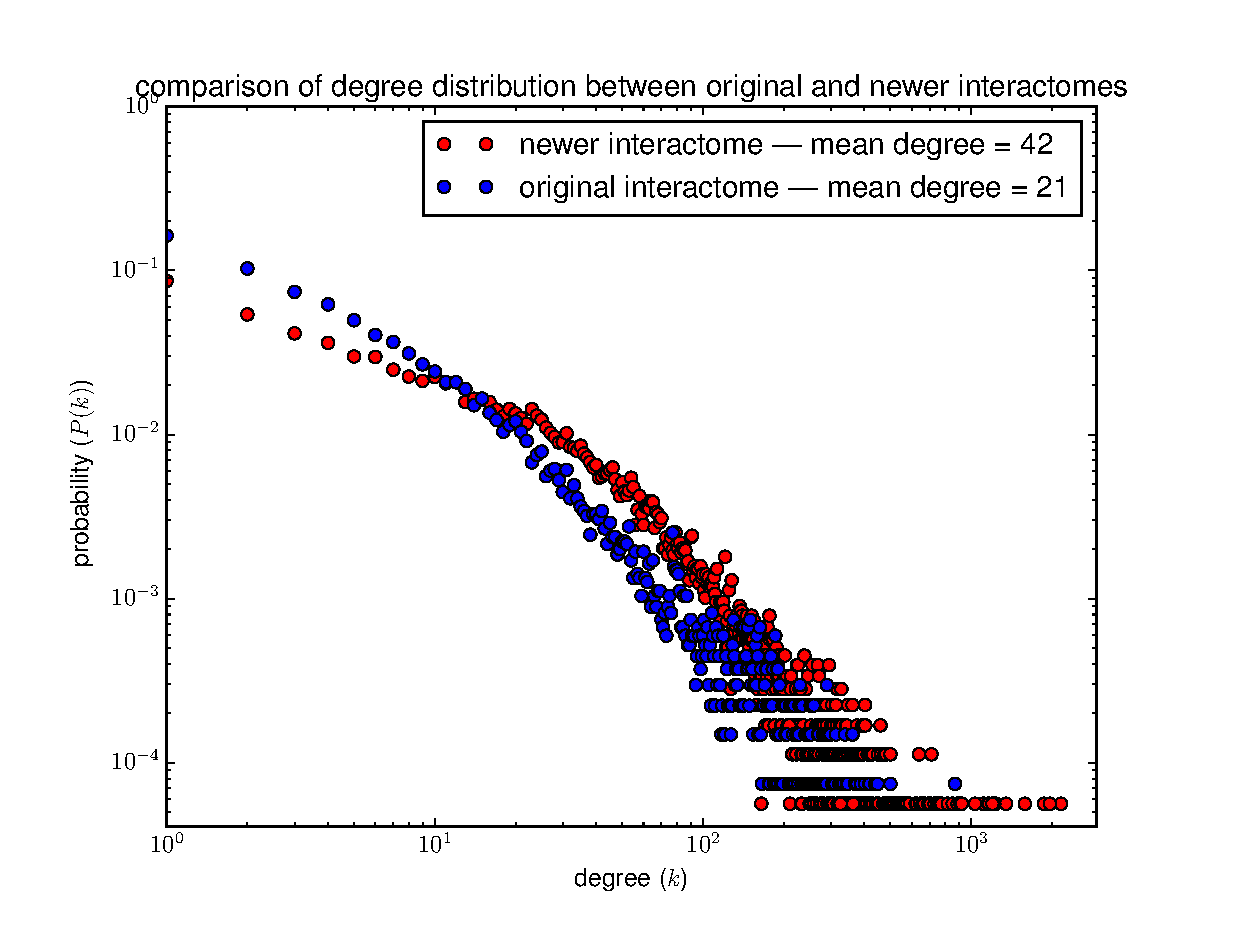
\includegraphics[scale=.36]{images/degree_distributions_comparison.eps}
		\caption{{\bf Degree distribution comparison.} ({\bf A}) The degree of a node $A$ in a graph is the number of nodes
		$B$ adjacent to $A$. Both the original interactome and the newer one are scale-free, i.e. their degree distribution
		follows a power law. This means that for a number $k$, $P(k)$, the probability that a node in the graph is of degree
		$k$ is given by $\alpha k^{-\gamma}$ with $\gamma$ the distribution parameter, and $\alpha = \zeta(\gamma)^{-1}$
		the regularization parameter. A power law is characterized by a few nodes being highly connected to the other ones
		(right part of the graph, with big values of $k$), whereas most nodes are connected to only a few other ones (left
		part of the graph, with small values of $k$). The newer interactome has a smaller $\gamma$ coefficient, meaning that
		a bigger proportion of nodes have a high degree, compared to the original one.
		({\bf B}) Cumulative degree distribution of both the original and the newer interactome. We observe easily the power
		law characteristic that even though degree can reach 2,000, almost all the interactome nodes have a degree $\leq 100$.
		\label{fig:degree distribution comparison}}
	\end{figure*}

	Despite the decrease in $z$-scores, we observe that general relative size has shifted towards right
	(Figure~\ref{fig:rel sizes comparison}).
	This is explained by the increase in the gene number, leading to a higher coverage of the disease genes, as well as
	the increase in density leading to a more connected graph, having therefore more connected subgraphs. Although,
	$z$-score maximum has dropped from 31.6 to 27.5, the mean $z$-score has increased from 6.2 to 6.4 due in part to the
	density increase in the region $z$-score $\in [10, 20]$.

	As well, average relative size for the given diseases has increased from $22\%$ to $32\%$ in the newer interactome,
	showing the better coverage allowed by the more recent version.

	The interpretation of Subsection~\ref{subsec:clustering of disease modules} still stand: diseases having a low $z$-score still
	have a low relative size, and diseases with a higher $z$-score have a higher relative size. So either the interactome is still
	too incomplete for these diseases, or they lie in very sparse regions of the interactome.

	Due to the graph density increase, the degree distribution has changed as well (Figure~\ref{fig:degree distribution comparison}).
	Both the original interactome and the new one are highly alike and comparable on their degree distribution. The most
	visible change is that the newer interactome contains more highly connected nodes which implies a mean twice as big.

	\begin{figure*}[!t]
		\hspace{-1.8cm}
		\vspace{-1cm}
		\includegraphics[scale=.35]{images/new_interactome_s_AB_histogram.eps}
		\caption{{\bf Disease pairs separation in the new interactome.} Adaptation of Figure~\ref{fig:s_AB histogram} on the
		newer interactome.
		({\bf A}) We observe that more than half of the disease pairs sharing no genes that had a negative $s_{AB}$ score
		in the original interactome now have a positive score, due to a decrease in $\langle d_A \rangle$ and $\langle d_B \rangle$
		because of the higher density of the newer interactome. ({\bf B}) We also observe that 29 disease pairs related by inclusion
		had a score right shift towards positive values.
		\label{fig:new interactome s_AB}}
	\end{figure*}

	Yet, the network is still scale-free, and its degree distribution still follows a power law, which is inherent to
	biological networks (coefficient 1.6 for the newer one versus 1.53 for the original one).\footnote{Determined by
	taking coefficient $\gamma$ in the relation $\log(P(k)) \sim -\gamma\log(k)$ found by a linear regression.}
	$\gamma$ is bigger than 1 and smaller than 3, which is considered
	relevant \citep{UnderstandingTheCellFunctionalOrganization,vidal2011interactome}.

	The 12 diseases which have a decrease of $z$-score below 1.6 is due to the increase of the interactome density implying
	that a subgraph taken at random tends to have a wider LCC at equal size.

	When applying the separation analysis on the newer interactome, we observe that non-overlapping diseases have a higher
	separation score in the newer interactome: from 710 disease pairs to 324 pairs having a $s_{AB} > 0$ score, i.e.
	so $54\%$ of the non-overlapping disease pairs increased their separation score above 0 (Figure~\ref{fig:new interactome s_AB}).

	We also observe that $6\%$ of the complete subset disease pairs decreased their separation score below 0, which is way
	less significant.

	More generally, separation scores have tightened around 0: $s_{AB}$ is in $[-3.2, 1.6]$ in the original interactome, and
	in the newer one, $s_{AB}$ is in $[-2.5, 1.1]$.

\section{Extension}
	\subsection{Subgraph largest connected component distribution}
	Figures~\ref{fig:zscore} and~\ref{fig:new interactome zscore} require a null hypothesis in order to define a $z$-score,
	being the random one. Those are computed as follows: if $S_D$ is the disease module associated with a given disease $D$,
	then its $z$-score is given by:
	\begin{equation}
		z\text{-score} = \frac {\abs {S_D} - \mu(S^{\text{rand}})}{\sigma(S^{\text{rand}})},
	\end{equation}
	with $\mu(S^{\text{rand}})$ and $\sigma(S^{\text{rand}})$ being respectively the mean and the
	standard deviation of the largest connected component size of a random subgraph of size $\abs D$
	in the interactome.

	These values are obtained by simulations: taking subgraphs at random of given size in the interactome yields a
	distribution $P(S^{\text{rand}})$ with a given mean $\mu(S^{\text{rand}})$ and standard deviation $\sigma(S^{\text{rand}})$
	(Figure~\ref{fig:Srand distribution}).

	\begin{figure}[!h]\centering
		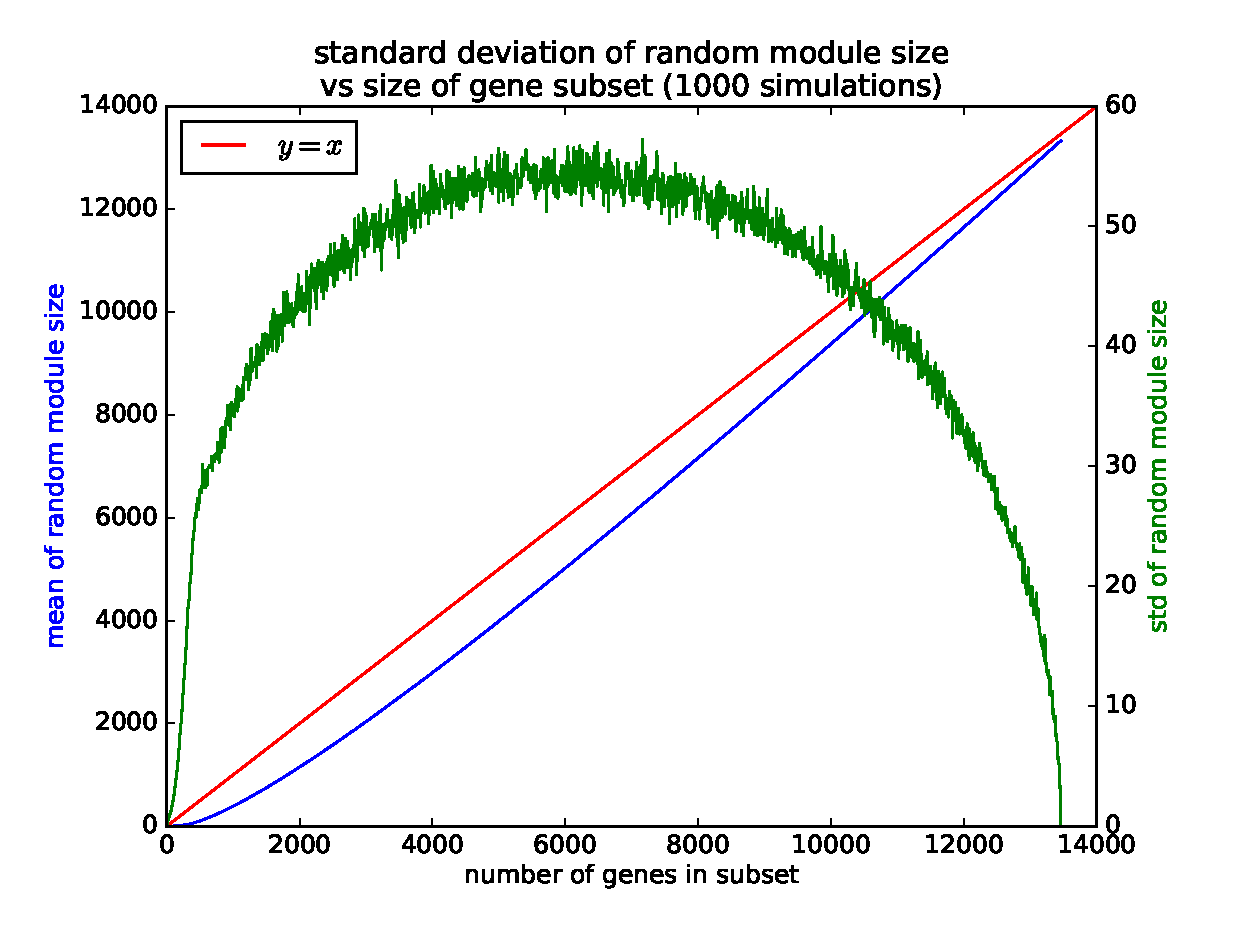
\includegraphics[width=.45\textwidth]{images/Srand_distribution_1000_sims.eps}
		\caption{{\bf $S^{\text{rand}}$ mean and standard deviation distribution.}
		With $10^3$ simulations per subgraph size, we obtain the distribution of the largest connected component size
		in the interactome. We observe that for subsets of small size $k$, the expected LCC size is significantly smaller than $k$
		whereas for subsets of big size $K$ (giant components), the expected LCC size is much closer to $K$.
		\label{fig:Srand distribution}}
	\end{figure}

	\subsection{Analytically determined probability density}
	In order to avoid simulation computation time, a probability mass function has been determined. For a graph $\Gamma = (V, E)$
	such that $\abs E = m$ and $\Lambda_k^m(V, \cdot)$, the set of all graphs having $V$ as vertex set, $m$ edges, and a LCC of size $k$,
	we define $p_k$, the probability that $\Gamma$ has LCC of size $k$ as:
	\begin{equation}
		p_k = \abs {\Lambda_k^m(V, \cdot)}/\binom {\binom {\abs V}2}m,
	\end{equation}
	which requires $\abs {\Lambda_k^m(V, \cdot)}$ to be computed. Yet, this set cardinality is defined by a recurrence relation
	(see proof in supplementary materials), which makes computations several orders of magnitude slower (even with dynamic programming
	and caching).

	A Python3 implementation is given in \texttt{source/lcc\_size/}.

\section{Conclusion}

\section{Materials and Methods}
	Inter-build (one of the programs from Inter-tools) requires datasets in the PSI-MITAB format, an extension of the
	PSI-MI format \citep{MITABFormat}, and outputs a tsv file.

	The outputted file by Inter-build and the interactome provided with the original paper both use Entrez gene IDs, they
	can therefore easily be merged. In order to merge these, the script \texttt{merger.py} has been written. As these two
	tsv files have a different format (different columns), only the gene IDs are outputted by \texttt{merger.py}.

\footnotesize
\bibliographystyle{apalike}
\bibliography{report}{}

\end{document}
